\chapter{Examples of simplifications}
\thispagestyle{empty}% no page number in chapter title page

In the examples below I used a mesh generated in the NavVis office from a dense point cloud. The mesh has 507277 vertices and 973168 faces.

\begin{sidewaysfigure}[ht]
    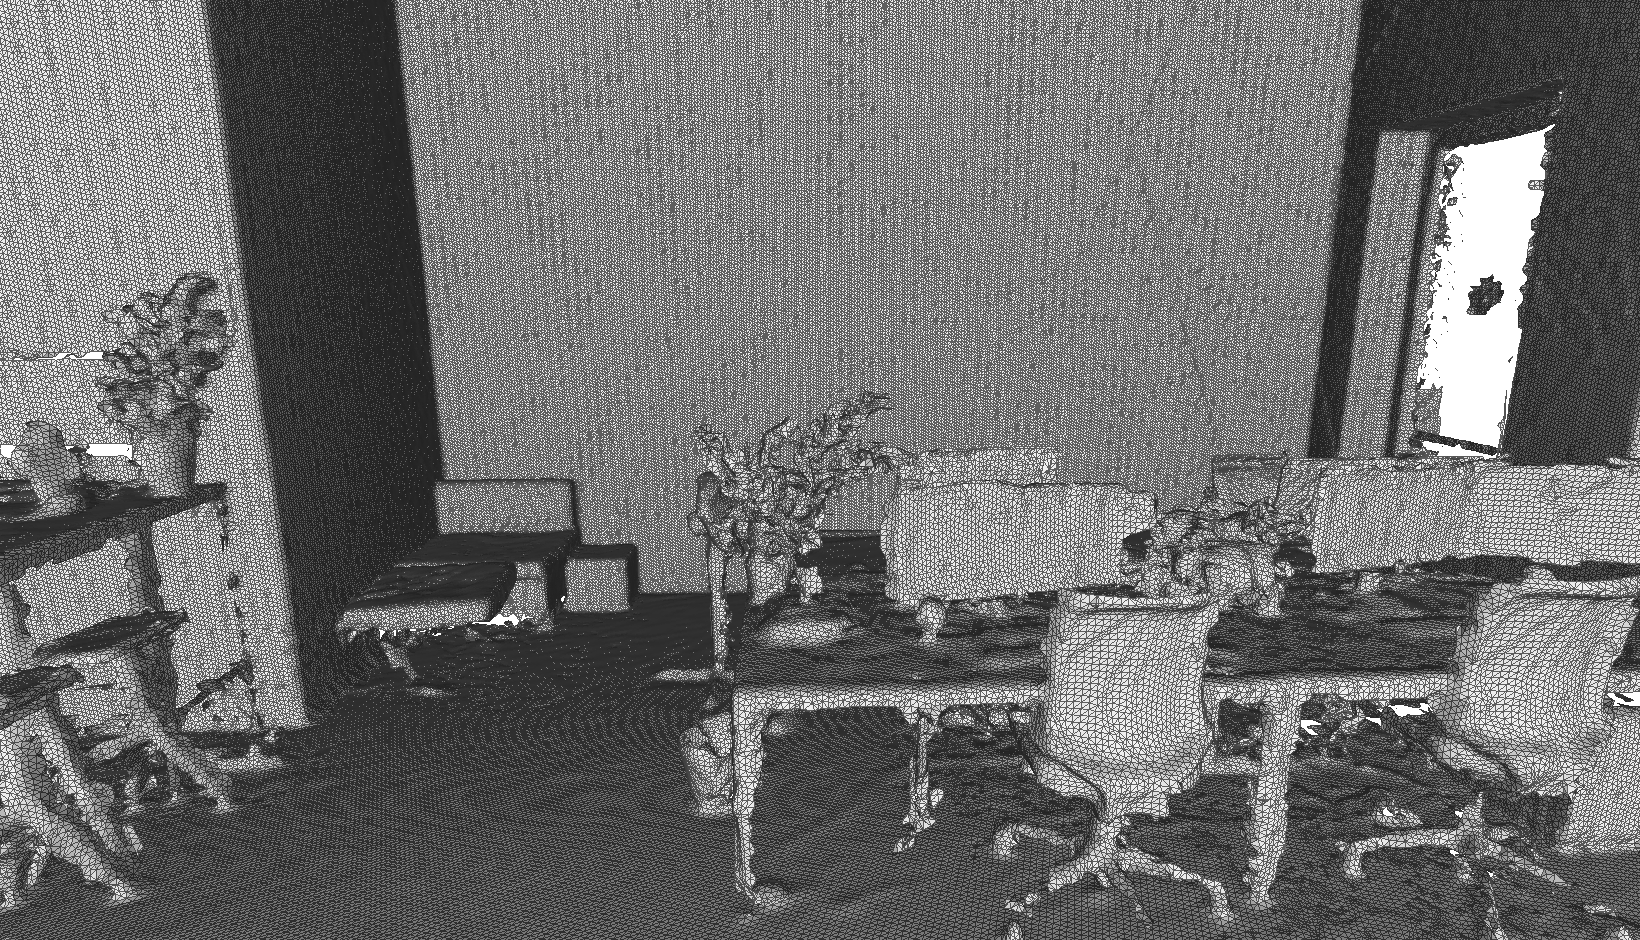
\includegraphics[width=20cm]{final_0}
    \caption{Original mesh with evenly distributed triangles.}
    \label{fig:final_0}
\end{sidewaysfigure}

\newpage
\begin{sidewaysfigure}[ht]
    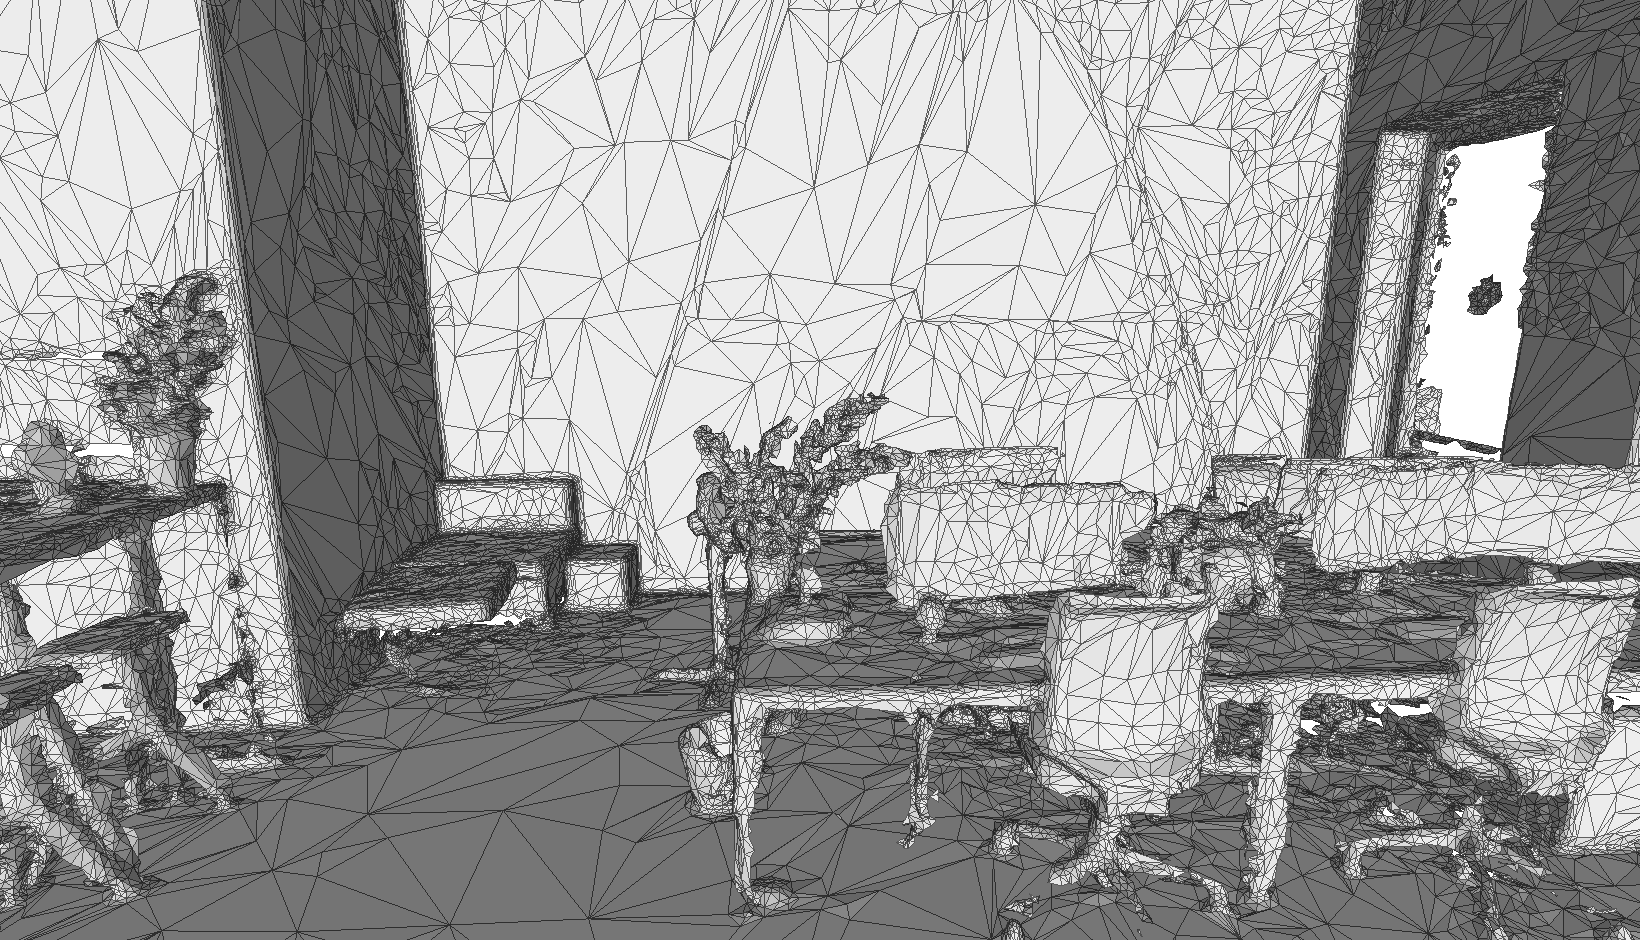
\includegraphics[width=20cm]{final_3}
    \caption{Simplified mesh to 15\% of the original using [geometry]}
    \label{fig:final_3}
\end{sidewaysfigure}

\newpage
\begin{sidewaysfigure}[ht]
    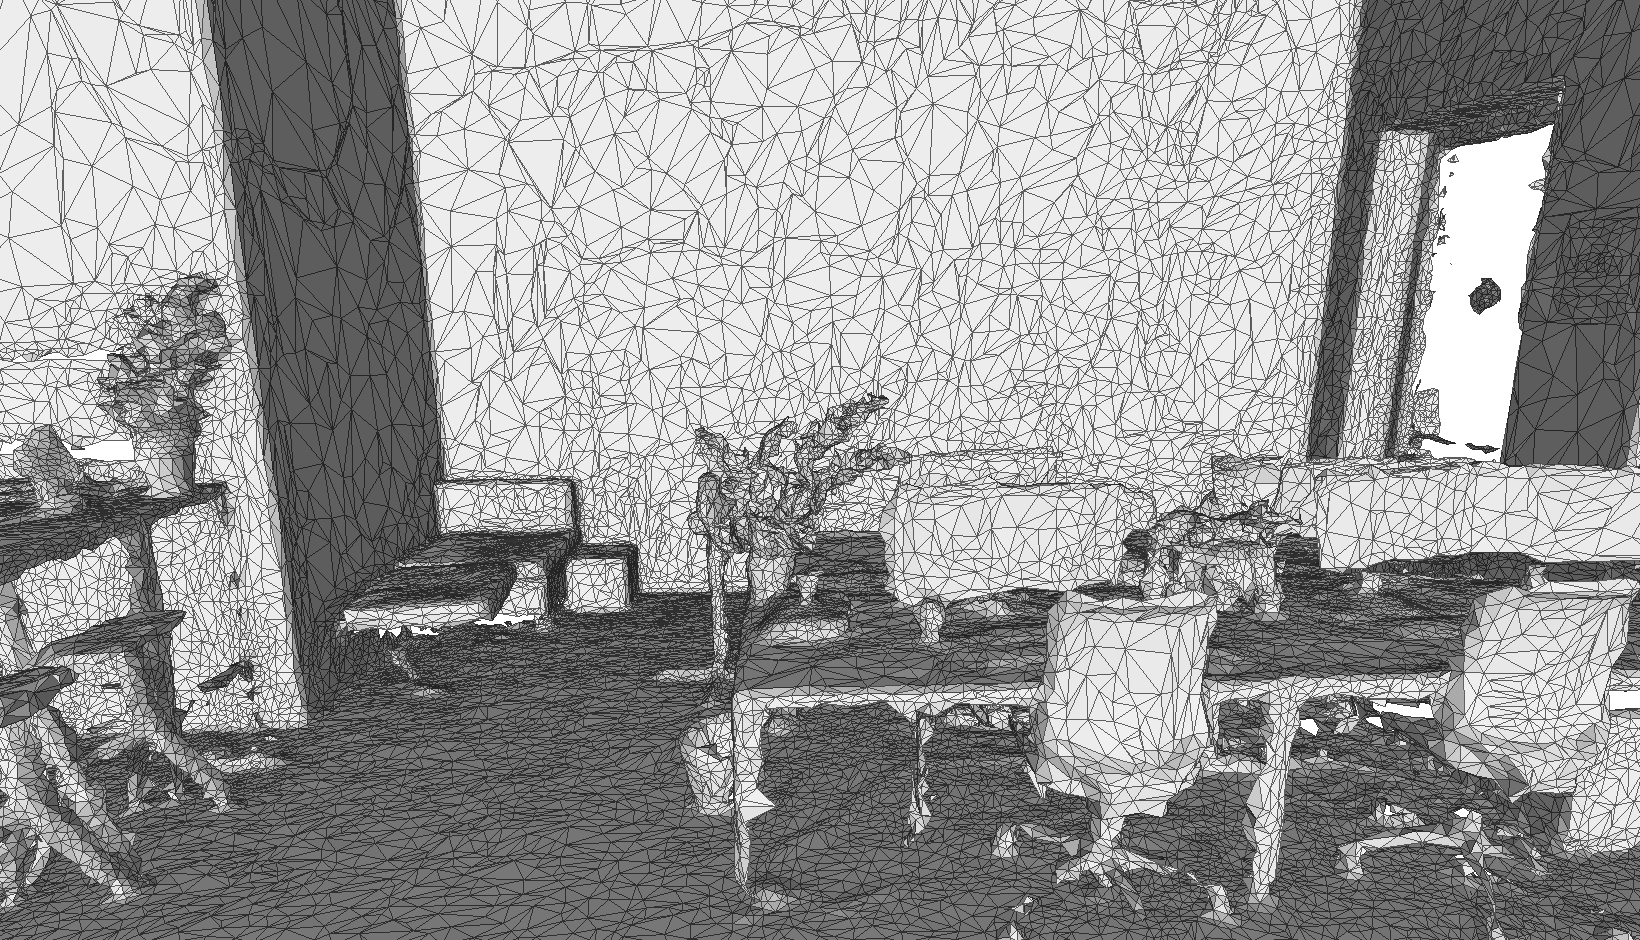
\includegraphics[width=20cm]{final_6}
    \caption{Simplified mesh to 15\% of the original using [geometry, color]}
    \label{fig:final_6}
\end{sidewaysfigure}

\newpage
\begin{sidewaysfigure}[ht]
    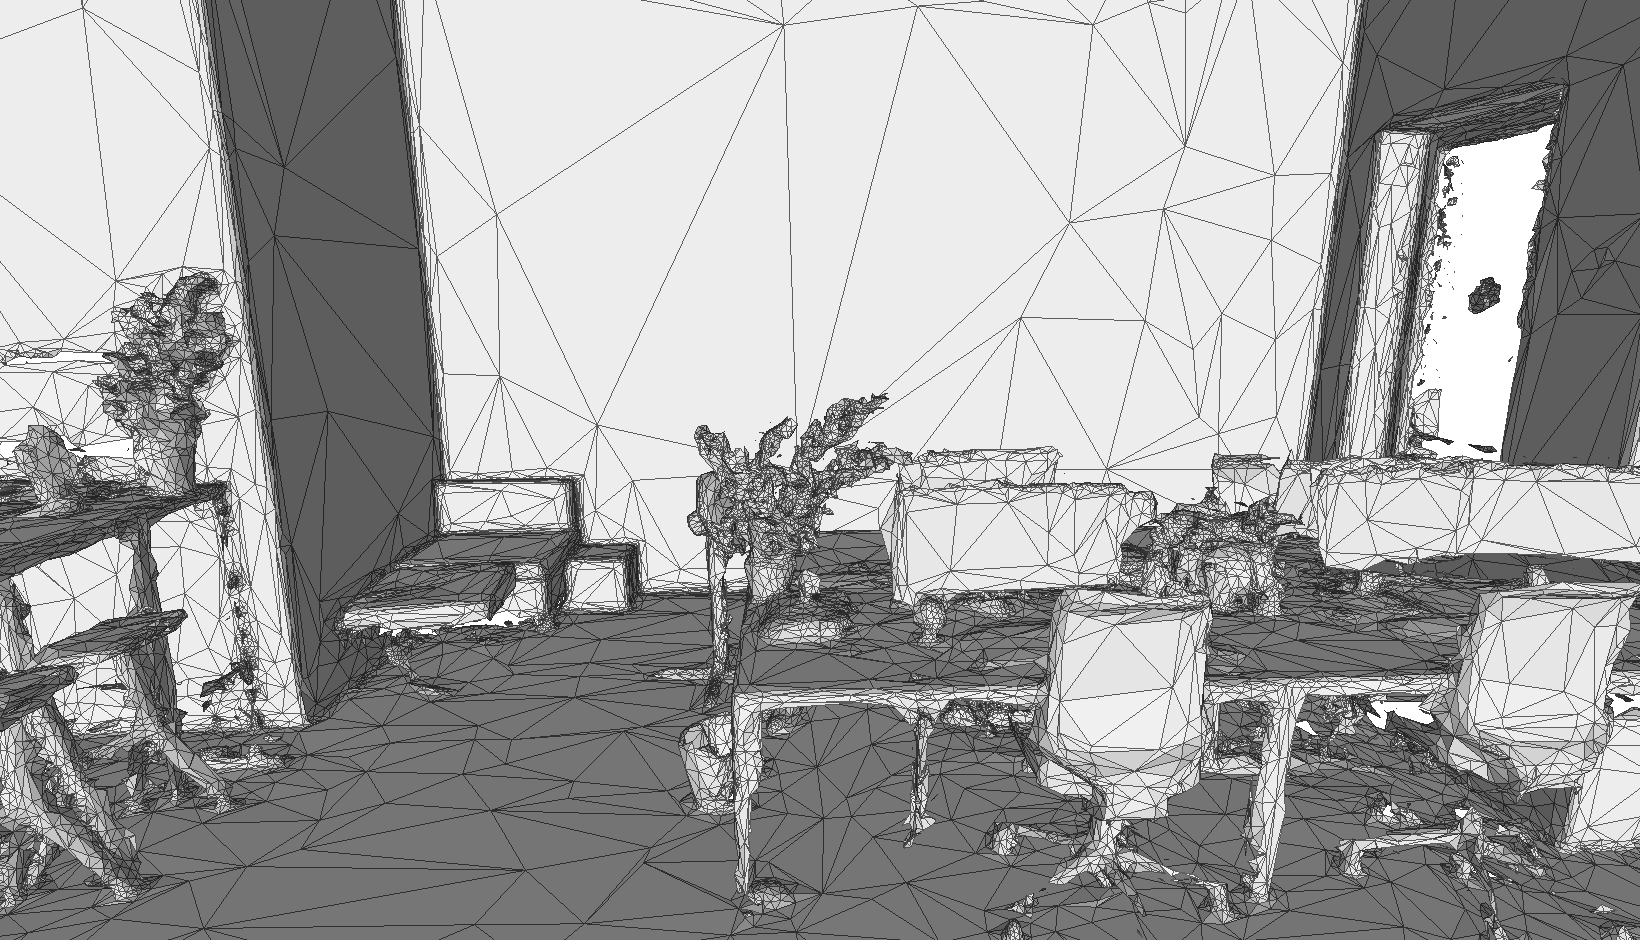
\includegraphics[width=20cm]{final_9}
    \caption{Simplified mesh to 15\% of the original using [geometry, color, normal]}
    \label{fig:final_9}
\end{sidewaysfigure}